\documentclass[slidestop,compress,mathserif,serif,notes=show]{beamer}
% Not to print overlays
% \documentclass[handout,slidestop,compress,mathserif,serif]{beamer}

% To use PSTricks
% \documentclass[slidestop,compress,mathserif,serif,xcolor=pst,dvips]{beamer}


\usepackage[utf8]{inputenc}
\usepackage{rfiw}
%\usepackage{ca}

\usepackage{algpseudocode}


\def\R{{\mathbb R}}
\def\C{{\mathbb C}}
\def\bS{{\mathbb S}}


\newcommand{\docTitle}{Track Clustering for Artist Disambiguation}
\newcommand{\subjectName}{Hack U}
\newcommand{\authors}{}

% PDF file properties
\title{\docTitle}
\hypersetup{
  pdfauthor={\authors},
  pdfsubject={\subjectName},
  pdfkeywords={rfiw, atelier, extraction, bibliographic, references}
}

\begin{document}

  % Hi, I'm Ramon and I'm going to present you a system that we implemented
  % last year for generating bibliographic references
  \begin{frame}
  \begin{center}
    %\footnotesize Facultat d'Informàtica de Barcelona\\
    %\small Grau en Enginyeria Informàtica\\

    \vspace*{2.2cm}
    
    \textbf{\small \subjectName}
    
    {\large \docTitle}

    \bigskip
    {\footnotesize February 2011}

    \vspace*{1.5cm}

  \end{center}
  \vspace{1cm}
\end{frame}



  %%%% MOTIVATION %%%%
  \section{Motivation and Goals}
  \begin{frame}
    \frametitle{\secname}
    \vspace*{0.5cm}
    \begin{enumerate}
      \item{}
      Multiple artists with the same name
      \item{}
      One single artist page/id
      \item{}
      But they play different music styles
      \item{}
      Tracks are tagged accordingly
      \item{}
      Solution: Cluster tracks by tag
    \end{enumerate}
    
  \end{frame}

  \begin{frame}
    \frametitle{Example}
    \vspace*{0.5cm}
    \begin{figure}
      \centering 
      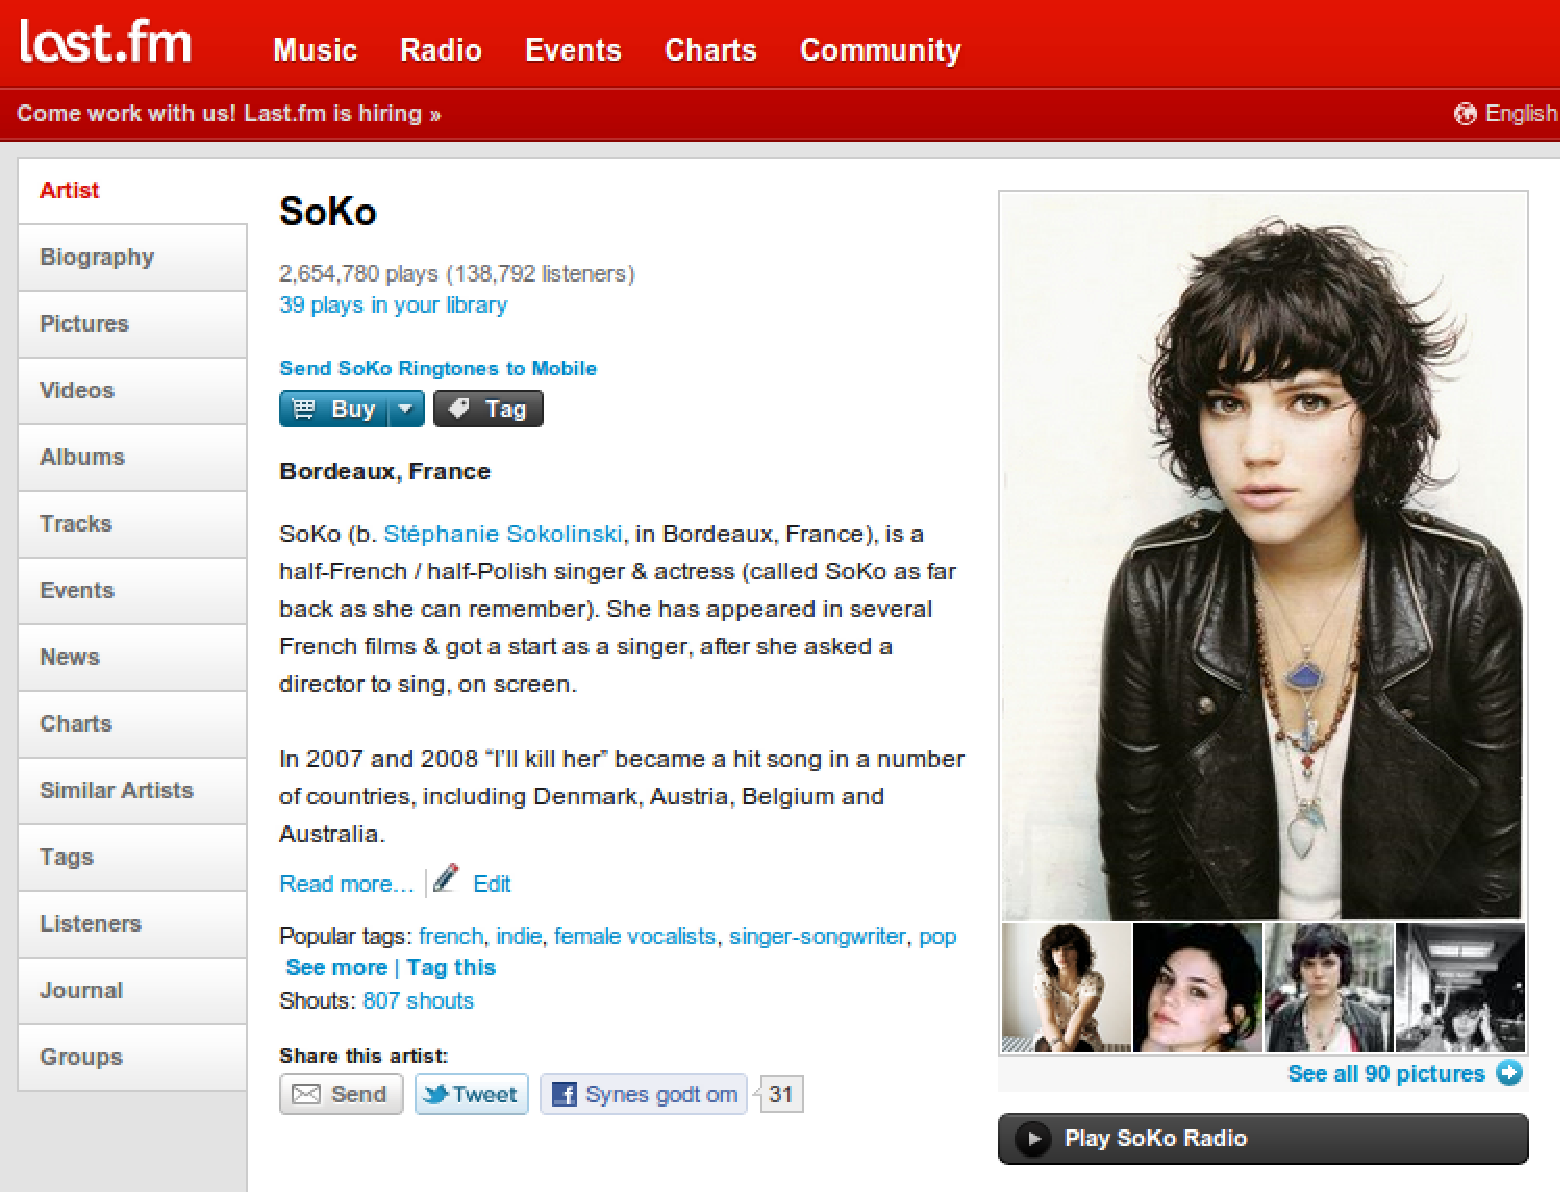
\includegraphics[width=0.7\textwidth]{figs/soko.pdf} 
      \label{fig:soko} 
    \end{figure}
    \begin{enumerate}
      \item{}
      Some songs: \texttt{french, female vocalist, cute, indie...}
      \item{}
      Some other songs: \texttt{instrumental, ambient, jazz...}
    \end{enumerate}
  \end{frame}


  
  \begin{frame}
    \frametitle{Overview}
    \vspace{0.5cm}
    \begin{figure}
      \centering 
      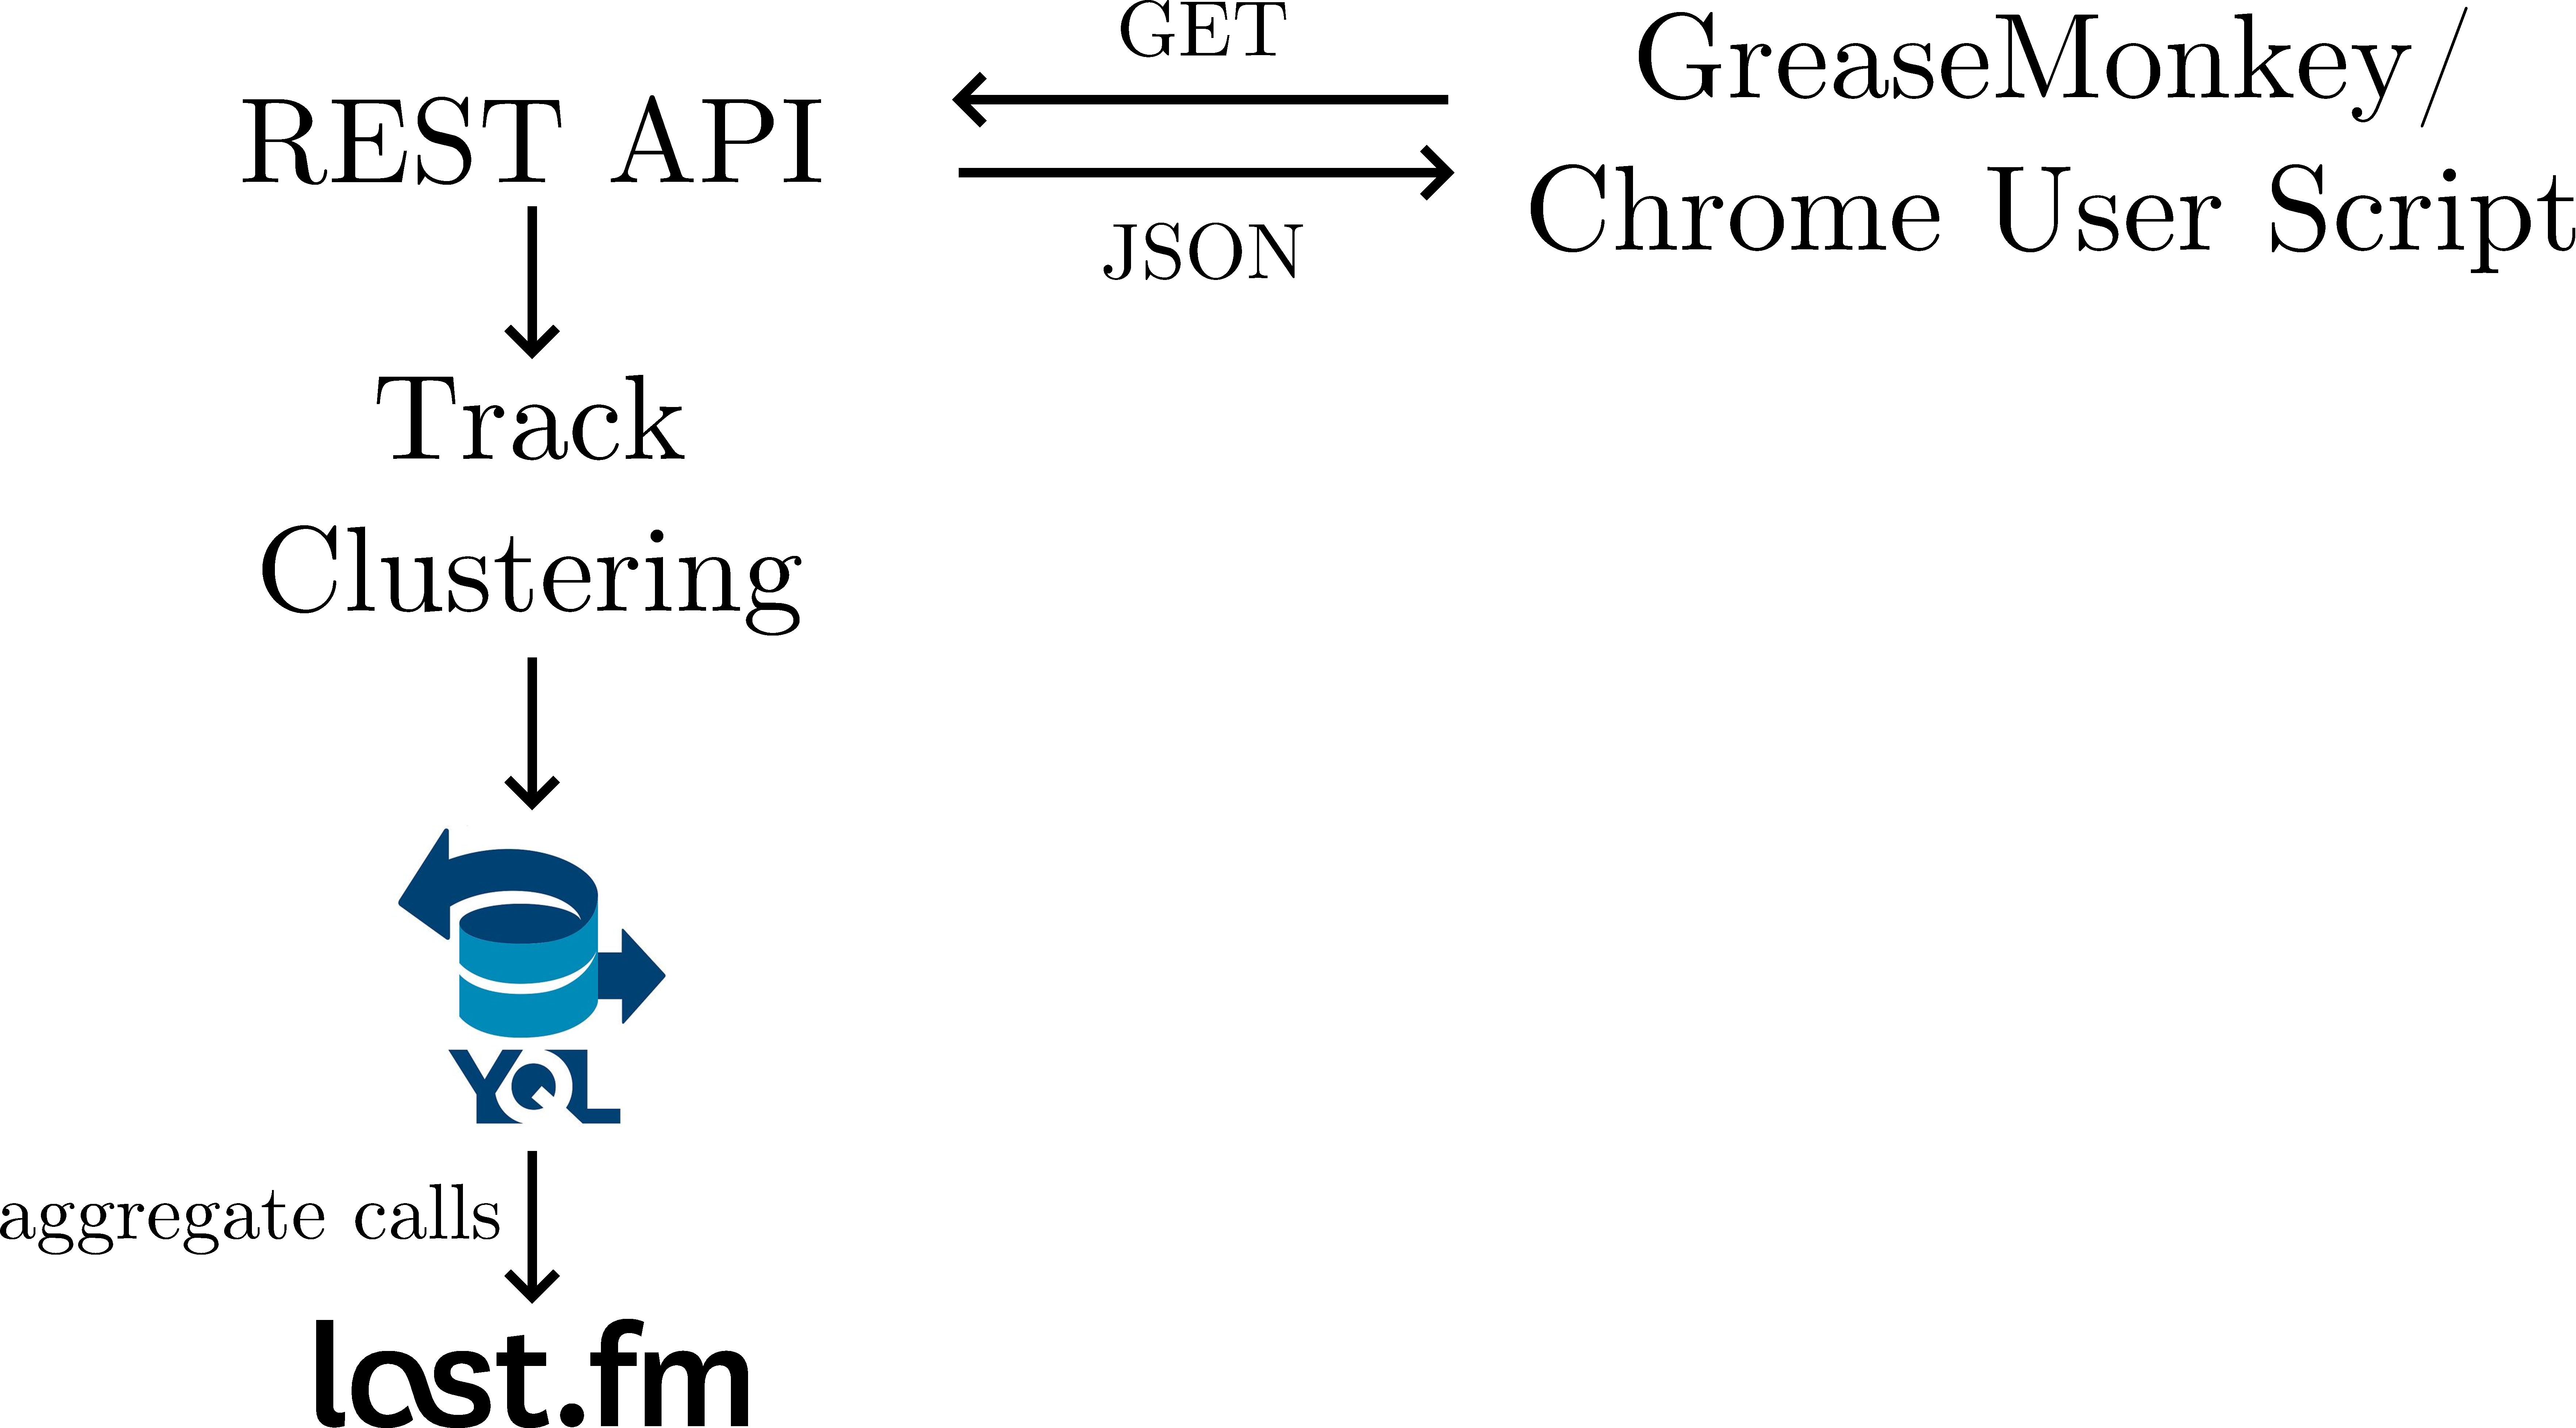
\includegraphics[width=0.9\textwidth]{figs/diagram.pdf} 
      \label{fig:diagram} 
    \end{figure}
  \end{frame}


  %%%% CONCLUSIONS %%%%
  \section{Thoughts and Conclusions}
  \begin{frame}
    \frametitle{\secname{}}
    \vspace{1cm}
    \begin{itemize}
      \item{}
      Clustering algorithm must be replaced\\
      \textcolor{gray}{Currently using hierarchical clustering with a threshold on the
      max. number of clusters and using complete linkage\\
      Other algorithms using frequent tag sets might be more appropiate}
      \item{}
      Only makes sense when applied during track streaming\\
      \textcolor{gray}{Chrome extension just for the sake of this demo}
    \end{itemize}
  \end{frame}

\end{document}

